\textbf{C: Programlama Aşaması }
\label{DokuzuncuBolum}

Tüm devrelerin montajı tamamlandı ve projenin programlama aşamasına geçildi. Bu aşamada ilk önce fare hareketlerinin analog değerleri serial monitörden okunarak hassasiyet değerlendirmesi maksatıyla tam değerleri bulundu. Arduino NANO devre kartı ise okunan değerleri projede kullanılan servo motorlara dikey ve yatay açısal bilgileri gönderecek şekilde programlandı. Tüm kodlamalar Arduino IDE programı vasıtasıyla Bilgisayardan USB kablo ile Arduino NANO Mikrodenetleyicisine aktarıldı.

\begin{figure}[H]
	\centering
	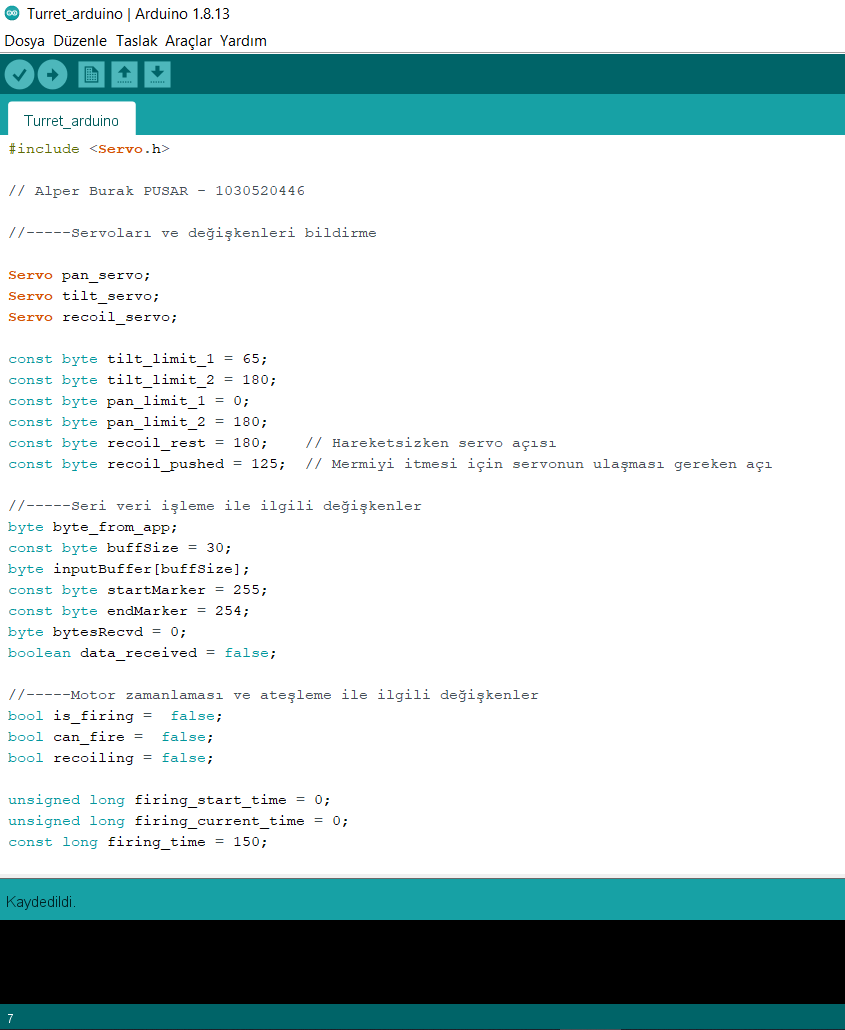
\includegraphics[width=120mm]{grafik/Kod 1.png}
	\label{fig:KodDM}
\end{figure}
\begin{figure}[H]
	\centering
	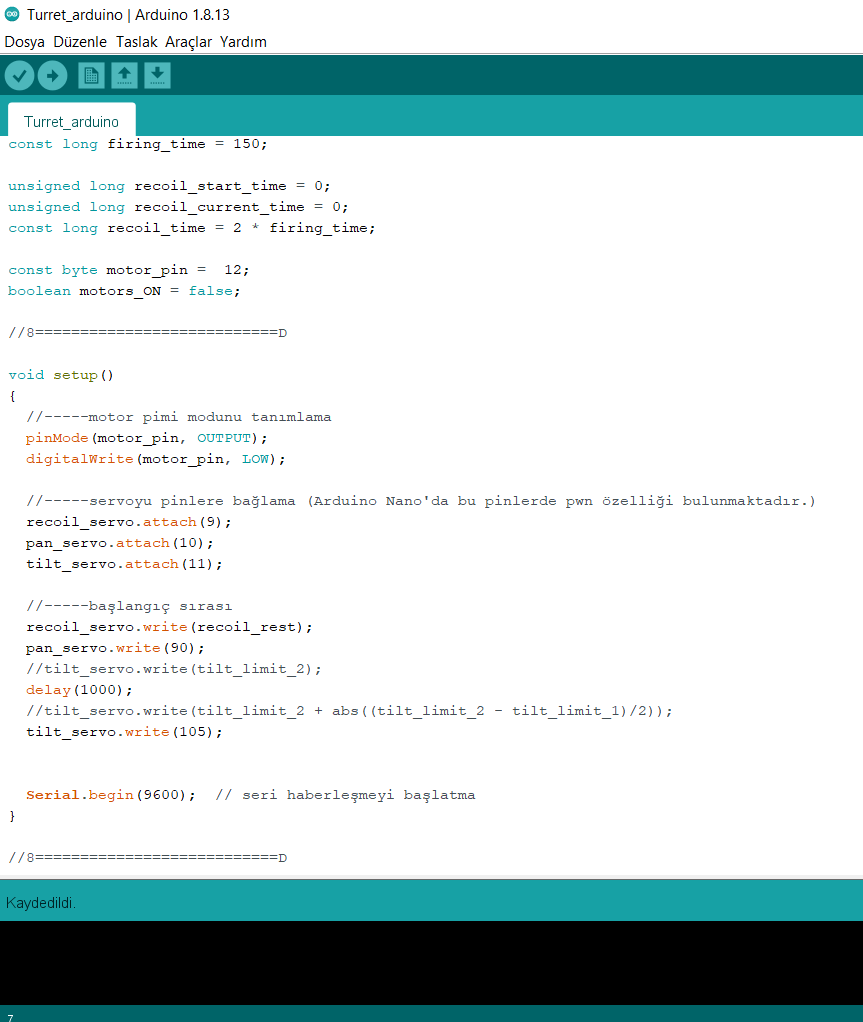
\includegraphics[width=120mm]{grafik/Kod 2.png}
	\label{fig:KodDM}
\end{figure}
\begin{figure}[H]
	\centering
	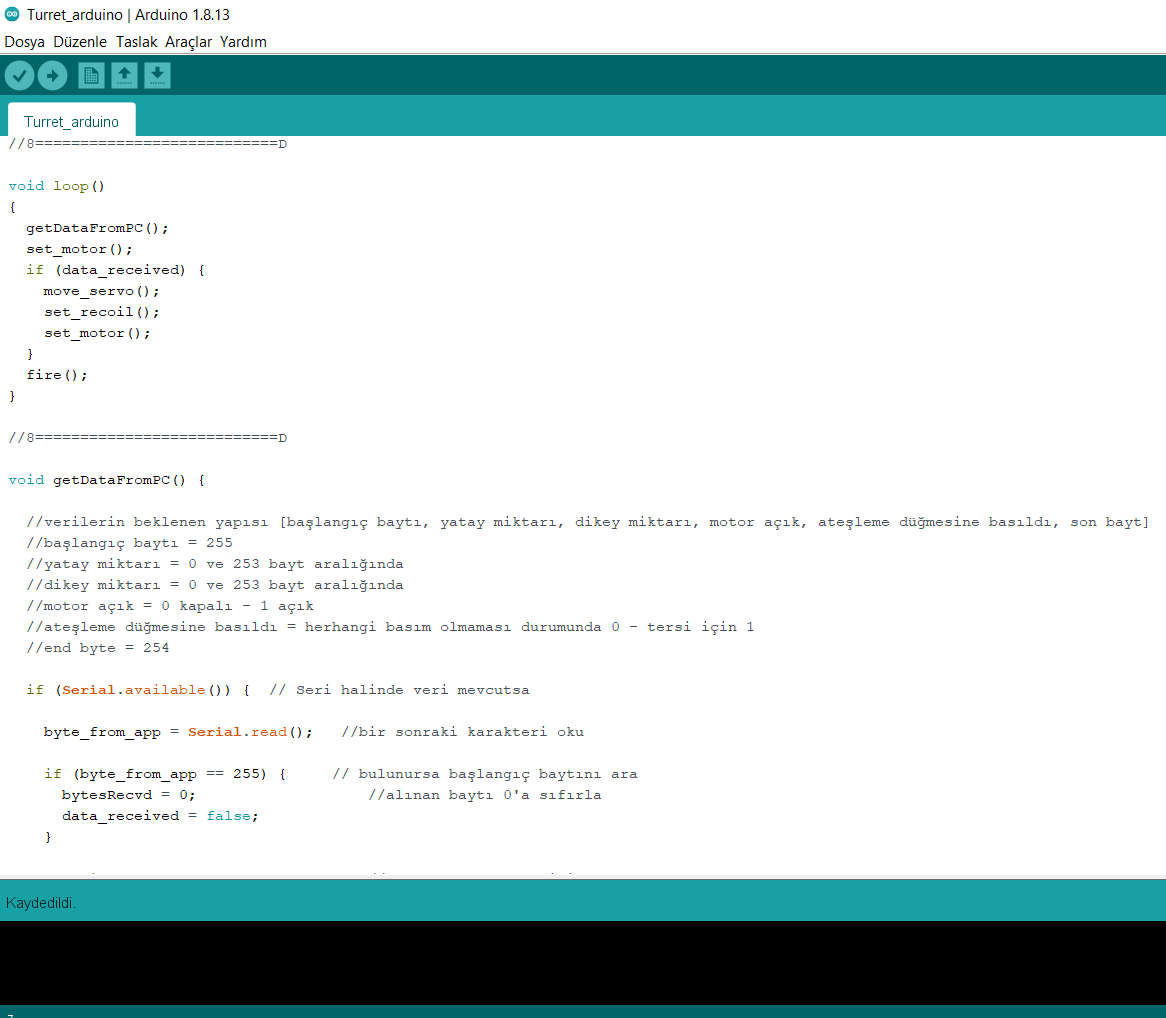
\includegraphics[width=120mm]{grafik/Kod 3.png}
	\label{fig:KodDM}
\end{figure}
\begin{figure}[H]
	\centering
	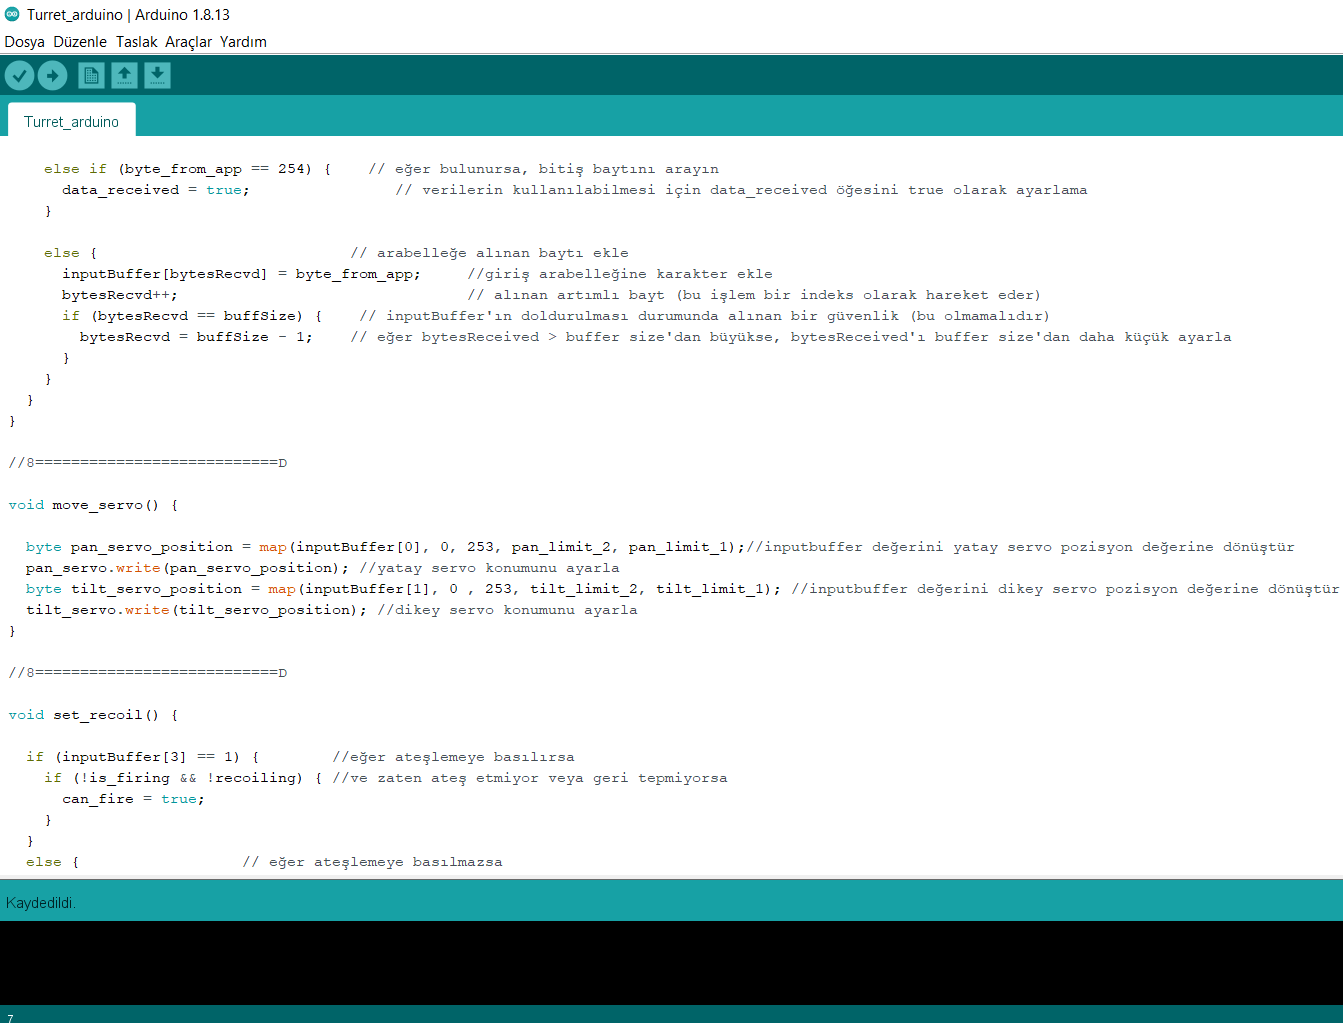
\includegraphics[width=120mm]{grafik/Kod 4.png}
	\label{fig:KodDM}
\end{figure}
\begin{figure}[H]
	\centering
	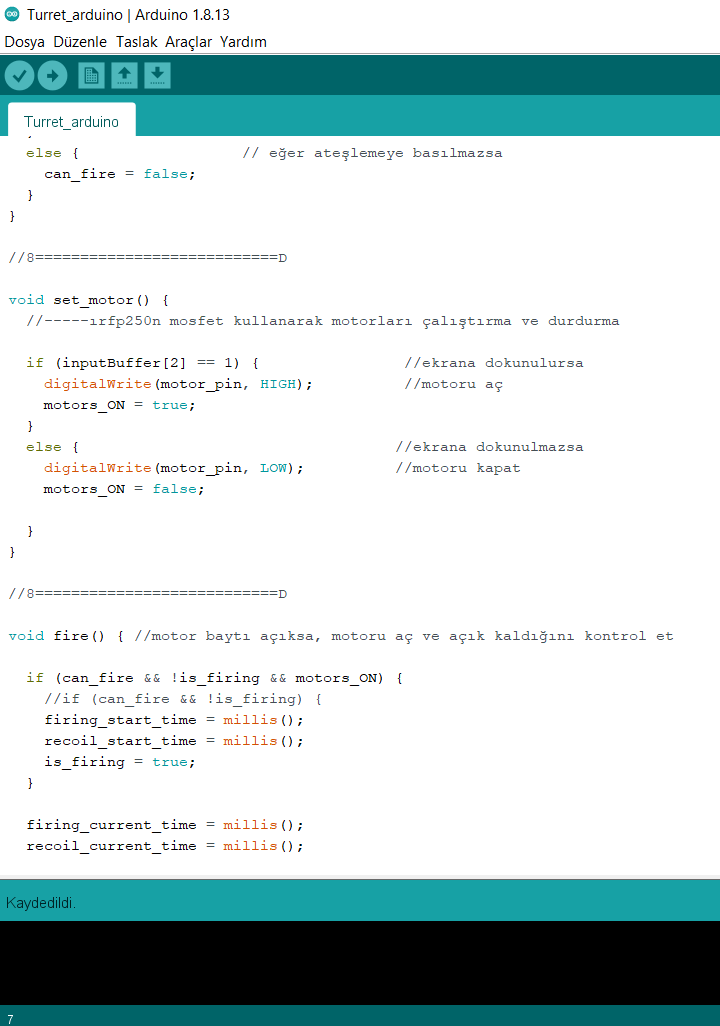
\includegraphics[width=120mm]{grafik/Kod 5.png}
	\label{fig:KodDM}
\end{figure}
\begin{figure}[H]
	\centering
	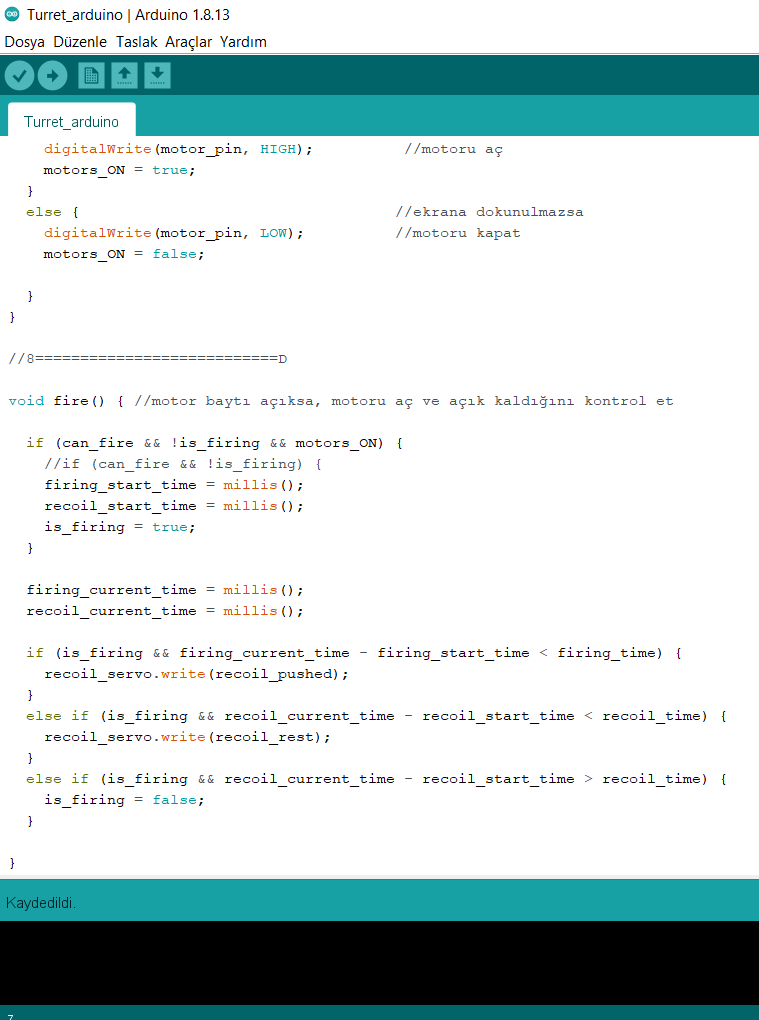
\includegraphics[width=120mm]{grafik/Kod 6.png}
	\label{fig:KodDM}
\end{figure}

\clearpage